\documentclass[11pt,a4paper]{article}
\usepackage[utf8]{inputenc}
\usepackage{amsmath}
\usepackage{amsfonts}
\usepackage{amssymb}
\usepackage{makeidx}
\usepackage{graphicx}
\usepackage{lmodern}
\usepackage{kpfonts}
\usepackage{xcolor}
\usepackage{cancel}
\usepackage{mathtools}
\usepackage{schemata}
\usepackage{cancel}
\providecommand{\abs}[1]{\lvert#1\rvert}%Sirve para colocar valores absolutos
\providecommand{\norm}[1]{\lVert#1\rVert}%Sirve para colocar módulo
\usepackage[left=2.00cm, right=2.00cm, top=2.00cm,bottom=2.00cm]{geometry}
\author{Harold Alessander Jhon Zambrano Quispe}
\title{SOLUCIONARIO DE LA TAREA 1}
\begin{document}
   \begin{titlepage}%Habilita una pagina sin enumerar.
	\begin{center}
	 {\huge \textbf{Universidad Nacional de Ingeniería}}\\
	 \vspace{3mm}
	  {\Large {Facultad de Ingeniería Eléctrica y Electrónica}}\\
	\vspace{-5mm}	 
	 \begin{figure}[h]
	 	\centering 
	 	
\includegraphics[scale=0.5]{Logo UNI}
	 \end{figure}
	 \vspace{-6mm}
	{\Large {Especialidad de Ingeniería de Telecomunicaciones}}\\
	\vspace{3mm}
	{\Large \textbf{"Solucionario del 2da Práctica Calificada"}}\\
	\vspace{8mm}
	\begin{flushleft}
	{\Large {\textbf{Curso}: Análisis de Señales y Sistemas}}\\
	\vspace{8mm}		
	{\Large {\textbf{Código del Curso}: EE410-M}}\\	
	\vspace{8mm}	
	{\Large {\textbf{Docente}: Manuel Arevalo Villanueva}}\\
	\vspace{8mm}	
	{\Large {\textbf{Alumno}: Harold Alessander Jhon Zambrano Quispe}}\\
	\vspace{8mm}	
	{\Large {\textbf{Código de Alumno}: 20191351B}}\\
	\end{flushleft}
	\vspace{10mm}
	{\Huge {\textbf{2021-I}}}\\
	\end{center}
\end{titlepage}
%Se debe compilar desde la funcion principal
	\section{\textbf{2.Sea la señal en tiempo discreto $X[n]=\dfrac{n+1}{2^n}. u[n-1]$. Calcule el valor de la energia $E[\infty]$}}{
	\Large{
	\begin{enumerate}
	\item[\textbf{.)}]
	\textbf{Solución:}\\
	\textbf{Importante: Energia discreta de una señal}\\
	\begin{eqnarray}	\label{EnergiaDiscretaSeñal}
	\boxed{E=\sum_{n=-\infty}^{\infty}{\vert X[n] \vert}^2}
	\end{eqnarray}
	\textbf{1er paso:}\\
	Como $X[n]=\dfrac{n+1}{2^n}. u[n-1]$\\
	Reemplazando en (\ref{EnergiaDiscretaSeñal})
	 $$E=\sum_{n=-\infty}^{\infty}{\vert \dfrac{n+1}{2^n}. u[n-1] \vert}^2$$
	 \textbf{2do paso:}\\
	 Graficando la señal u[n-1]
	\begin{center}
	\begin{figure}[h]
	 \centering 
	\includegraphics[scale=0.75]{ESCALONUNITARIODESPLAZADO}
	\caption{Gráfica de u[n-1])}	\label{ESCALONUNITARIODESPLAZADO}
	\end{figure}
	\end{center} 
	\begin{equation*}
	u[n-1]=
	\begin{cases}
0 & \text{;si $n < 1 $}\\
1 & \text{;si $n \geq 1$}
\end{cases}
	\end{equation*}
	De la grafica(\ref{ESCALONUNITARIODESPLAZADO})
,se verifica que para $n<1$ el $u(n-1)$ toma el valor de 0, entonces:
	$$E=\sum_{n=1}^{\infty}{\vert \dfrac{n+1}{2^n}\vert}^2$$
	$$E=1+{(\dfrac{3}{2^2})}^2+{(\dfrac{4}{2^3})}^2+{(\dfrac{5}{2^5})}^2+...$$
	\begin{center}
	$\therefore$ \boxed{E=\dfrac{53}{27}}
	\end{center}
	\end{enumerate}
	}}
	\section{\textbf{Sea la señal continua}}{
	\Large{
	\begin{enumerate}
	\item[\textbf{}]
	\begin{equation*}
	f(t) =
\begin{cases}
0 & \text{si $t < 0 $}\\
1-t^2 & \text{si $0 \leq t<1$}\\
5-2t & \text{si $1 \leq t<2$}\\
0 & \text{si $2 \leq t $}
\end{cases}
\end{equation*}
	\textbf{Si se cumple lo siguiente: $$f^{'}(t)=a-\delta (t)+b \delta (t-1) +c \delta (t-2) +d u_1(t)+e u_1(t-1)+f u_o(t-2)$$
	Calcule el valor de $a+b+c+d+e+f$}\\
	 \textbf{Solución:}\\
	 \textbf{1er paso:} Graficando f(t)
	 \begin{figure}[h]
	 \centering 
	\includegraphics[scale=0.75]{GRÁFICA4FT}
	\caption{Gráfica de f(t)}
	\label{GRÁFICA4FT}
	\end{figure}\\
	 A partir de la gráfica podemos encontrar lo siguiente:\\
	Para  $0 \leq t<1$:
	$$u(t)-u(t-1)$$	
	Para $1 \leq t<2$:
	$$u(t-1)-u(t-2)$$
Entonces, a partir de la función que nos dan y lo anterior, encontraremos el f(t) en función del escalonado
	$$f(t)=(1-t^2) (u(t)-u(t-1))+ (5-2t)(u(t-1)-u(t-2))$$
Operando y desarrollando, obtenemos lo siguiente
	$$f(t)=u(t)-u(t)t^2-u(t-1)+t^2u(t-1)+5u(t-1)-2tu(t-1)-5u(t-2)
	+2tu(t-2)$$
	Derivando y aplicando $\delta_{t_0}(t)=u_{t_o}^{'}(t)$
	$$f^{'}(t)=(1-t^2)\delta(t)+(t^2-2t+4)\delta(t-1)+(2t-5)\delta(t-2)-2tu(t)+(2t-2)u(t-1)$$
	$$+2u(t-2)$$
	Aplicando la siguiente propiedad $f(t)\delta(t-a)=f(a)\delta(t-a)$
	$$f^{'}(t)=\delta(t)+3\delta(t-1)-\delta(t-2)-2tu(t)+2tu(t-1)-2u(t-1)+2u(t-2)$$
	Aplicando la siguiente propiedad $ u_a(t)=\dfrac{t^a}{a!}u(t)$
	\begin{eqnarray}
	\label{u1}
	\cdot u_1(t)=\dfrac{t^1}{1!}u(t)
	\end{eqnarray}
	
	\begin{eqnarray}
	\label{ut-1}
	\cdot u_1(t-1)=\dfrac{(t-1)^1}{1!}u(t-1)=(t-1)u(t-1)
	\end{eqnarray}
	
	\begin{eqnarray}
	\label{u0}
	\cdot u_0(t-2)=\dfrac{(t-2)^0}{0!}u(t-2)=u(t-2)
	\end{eqnarray}
	Continuando con $f^{'}(t)$ y reemplazando (\ref{u1}) y (\ref{u0})
	$$f^{'}(t)=\delta(t)+3\delta(t-1)-\delta(t-2)-2u_1(t)+2(t-1+1)u(t-1)-2u(t-1)+2u_0(t-2)$$
	$$f^{'}(t)=\delta(t)+3\delta(t-1)-\delta(t-2)-2u_1(t)+2(t-1)u(t-1)+ \cancel{2u(t-1)}- \cancel{2u(t-1)}$$
	$$+2u_0(t-2)$$
	Reemplazando (\ref{ut-1})
	$$\boxed{f^{'}(t)=\delta(t)+3\delta(t-1)-\delta(t-2)-2u_1(t)+2u_1(t-1)+2u_0(t-2)}$$
	Comparando con el siguiente dato del problema:
	$$f^{'}(t)=a-\delta (t)+b \delta (t-1) +c \delta (t-2) +d u_1(t)+e u_1(t-1)+f u_o(t-2)$$
	Obtenemos los valores a,b,c,d,e,f\\
	$$a=1 , b=3, c=-1, d=-2 , e=2, f=2$$
	Finalmente, calculando lo pedido por el problema\\
	\begin{center}
	$\therefore$ \boxed{a+b+c+d+e+f=5}
	\end{center}
	\end{enumerate} 
	}}
	\section{\textbf{5.Considere la señal discreta $x[n]= 1- \sum_{k=3}^{n=\infty} \delta[n-1-k]$. Determine los valores de los enteros M y $n_o$ de tal manera que x[n] se exprese como $x[n]=u[Mn-n_0]$. Dar como respuesta $M+n_0$.}}{
	\Large{
	\begin{enumerate}
	\item[\textbf{.}]
	\textbf{Solución:}\\
	\textbf{1er paso:} \\
	$$x[n]= 1- \sum_{k=3}^{n=\infty} \delta[n-1-k]$$
	$$x[n]= 1- \delta[n-4]-\delta[n-5]-\delta[n-6]-\delta[n-4]-...$$
	\textbf{2do paso:}\\
	Graficando x[n]:
	$\cdot$ Graficando $- \delta[n-4]-\delta[n-5]-\delta[n-6]-\delta[n-4]-...$
	\begin{center}
	\begin{figure}[h]
	 \centering 
	\includegraphics[scale=0.7]{DELTAS1}
	\label{DELTAS1}
	\end{figure}
	\end{center}
	\newpage
	Graficando $$x[n]= 1- \delta[n-4]-\delta[n-5]-\delta[n-6]-\delta[n-4]-...$$\\
	\begin{center}
	\begin{figure}[h]
	 \centering 
	\includegraphics[scale=0.7]{Xn}
	\label{Xn}
	\end{figure}
	\end{center}
	A partir del escalón unitario, obtendremos lo siguiente:\\
	\begin{center}
	\begin{figure}[h]
	 \centering 
	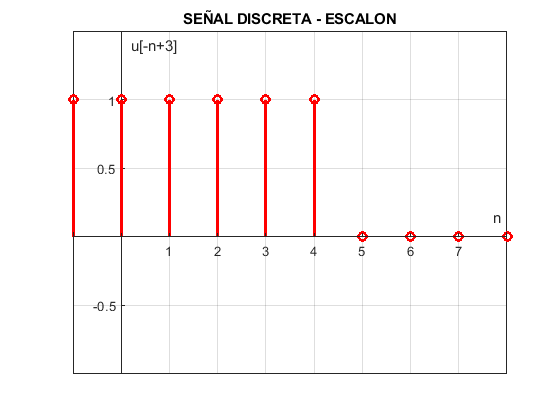
\includegraphics[scale=0.7]{UNMAS3}
	\label{UNMAS3}
	\end{figure}
	\end{center}
	$$x[n]=u[Mn-n_o]=u[-n-(-3)]$$
	$$M=-1 y n_0=-3$$
	\begin{center}
	$\therefore$ \boxed{M+n_o=-4}
	\end{center}
	\end{enumerate}
	}}
\end{document}









